Những mối quan hệ của bối cảnh bị giới hạn cần được quản lý chặt chẽ để hoạt động độc lập, nhất quán và linh hoạt. Do đó, chúng ta cần phải ghi lại các mối quan hệ thông qua việc sử dụng bản đồ bối cảnh. \emph{Bản đồ bối cảnh (Context Maps)} là sự thể hiện trực quan của hệ thống, thể hiện các thành phần và mối quan hệ giữa các thành phần.

\begin{figure}[H]

\centering

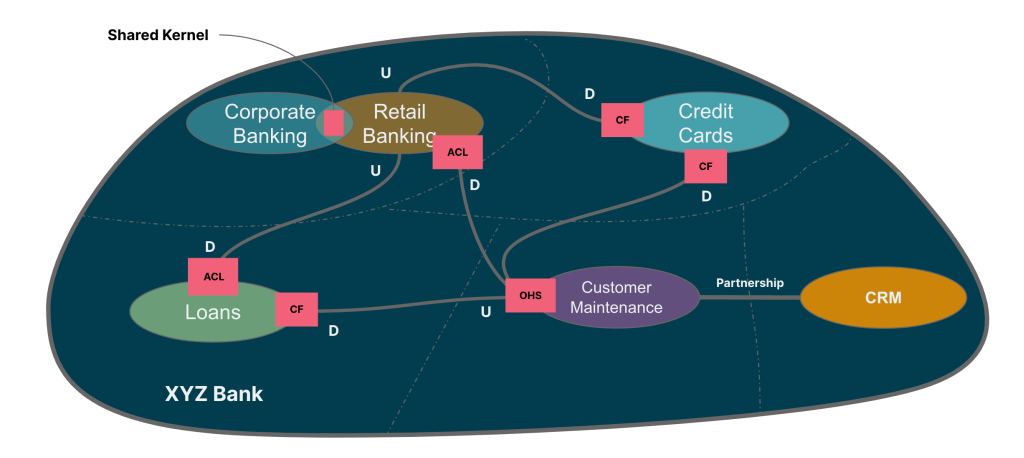
\includegraphics[scale = 0.4]{pictures/_vi_du_ban_do_boi_canh_trong_1_ngan_hang/main.drawio.png}

\caption{Ví dụ bản đồ bối cảnh trong 1 ngân hàng}

\end{figure}

\subsubsection{Áp dụng bản đồ bối cảnh}

\begin{itemize}

\item Do user - service và invoice - service cần sử dụng uuid của tct - demo nên tct - demo là OHS và user - service, invoice - service cần tuân thủ.

\item Tiếp theo, user - service cung cấp invoice - service, và invoice - service cung cấp report - service do sử dụng kiến trúc lục giác (Hexagonal Architecture) nên bối cảnh bị giới hạn hạ lưu là ACL.

\end{itemize}

\begin{figure}[H]

\centering

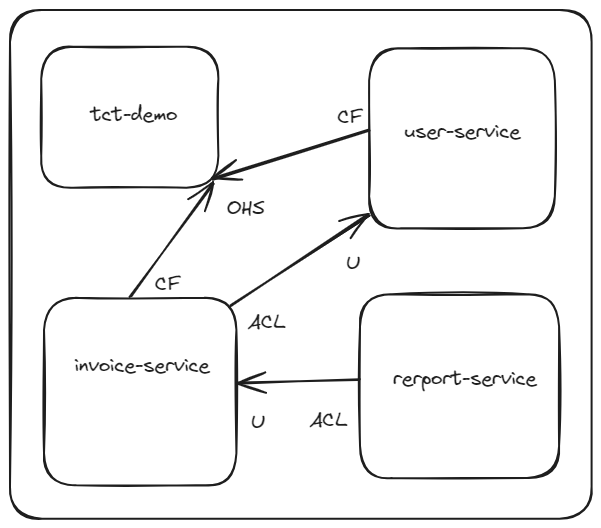
\includegraphics[scale = 0.4]{pictures/_ap_dung_ban_do_boi_canh/freelancer.main.excalidraw.png}

\caption{Áp dụng bản đồ bối cảnh trong đồ án}

\end{figure}